\documentclass[tikz,border=10pt]{standalone}
\begin{document}
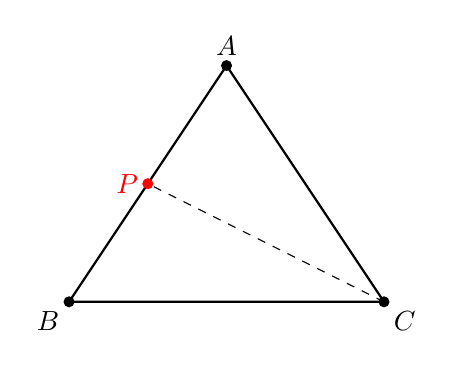
\begin{tikzpicture}

    % Define the points
    \coordinate (A) at (0, 3);
    \coordinate (B) at (-2, 0);
    \coordinate (C) at (2, 0);
    \coordinate (P) at (-1,1.5);

    % Draw the triangle ABC
    \draw[thick] (A) -- (B) -- (C) -- cycle;

    % Draw the point P
    \fill[red] (P) circle (2pt) node[left] {$P$};

    
    \draw[dashed] (C) -- (P);
    

    % Label the vertices
    \fill[black] (A) circle (2pt) node[above] {$A$};
    \fill[black] (B) circle (2pt) node[below left] {$B$};
    \fill[black] (C) circle (2pt) node[below right] {$C$};


\end{tikzpicture}
\end{document}